\chapter{Implementacja}
W niniejszym rozdziale opisano proces, którego celem było zaimplementowanie platformy spełniającej postawione wcześniej wymagania funkcjonalne oraz niefunkcjonalne. 
W procesie tym wystąpiły wszystkie kluczowe kroki, począwszy od konfiguracji środowiska, przez rozwój aplikacji backendowej i frontendowej, aż po integrację z systemami zewnętrznymi oraz konfigurację kontenerów Dockerowych. Lektura tego rozdziału powinna pozwolić na zapoznanie się ze szczegółami implementacji, uwagami dotyczącymi użytych technologii, narzędzi oraz metodami, które umożliwiły realizację tak założonego projektu.

W rozdziale omówione zostaną aspekty techniczne implementacji, w tym struktura repozytoriów kodu, konfiguracja środowiska developerskiego, użyte frameworki i biblioteki, oraz zagadnienia związane z budową i wdrożenia aplikacji. Zaznaczono w nim główne decyzje architektoniczne, które wpłynęły na projektowanie aplikacji oraz integrację z systemami zewnętrznymi, w tym bazami danych, serwerami aplikacji oraz kontenerami Dockerowymi.

Podczas implementacji, szczególną uwagę poświęcono skalowalności aplikacji, zapewnieniu bezpieczeństwa danych oraz optymalizacji wydajności. Każdy z komponentów systemu – zarówno backend jak i frontend – został zaprojektowany w sposób umożliwiający łatwą rozbudowę oraz integrację z dodatkowymi usługami w przyszłości.


\section{Podział logiczny}
\subsection{Komponenty systemu}
Zgodnie z założeniami co do architektury, podczas implementacji stworzono główne moduły systemu: frontend oraz backend (patrz podrozdział~\ref{subsec:ZarysArchitektury}).

Frontend, zbudowany w React, odpowiada za prezentację danych i interakcję z użytkownikami. Podzielono go na moduły odpowiadające różnym domenom funkcjonalnym. Moduł blockchain prezentuje dane związane z blockchainami Bitcoin, Ethereum i Solana, w tym szczegóły transakcji, bloków oraz kont. Ten moduł zawiera podkomponenty obsługujące wyszukiwanie oraz wyświetlanie szczegółowych informacji. Moduł kryptowalut zarządza kategoriami kryptowalut, danymi historycznymi, rynkiem globalnym oraz rankingami. Dodatkowo frontend oferuje widoki użytkownika, takie jak logowanie, rejestracja oraz strona główna. Komunikacja z backendem odbywa się za pomocą biblioteki axios, z uwierzytelnianiem opartym na tokenach JWT przechowywanych w \texttt{localStorage}.

Backend systemu został zaimplementowany w Spring Boot 3 przy użyciu Javy 21. Jest to centralny komponent systemu, który integruje funkcjonalności związane z logiką biznesową, bazą danych oraz zewnętrznymi dostawcami informacji. Backend udostępnia API REST dla frontendu i obsługuje kilka kluczowych domen, takich jak kryptowaluty, NFT oraz zasoby zewnętrzne. Moduł kryptowalut oferuje funkcje zarządzania kategoriami, danymi historycznymi oraz danymi rynkowymi. Moduł NFT zarządza tokenami, kolekcjami oraz ich statystykami. Backend również integruje dane blockchainowe, takie jak transakcje i bloki, które są dynamicznie pobierane z zewnętrznych API, takich jak Etherscan czy CoinMarketCap. Ponadto backend wywołuje dedykowane skrypty w Node.js w celu realizacji zaawansowanych operacji blockchainowych, takich jak symulacje transakcji i airdropy oraz skrypt w kontenerze Pythonowym, tak aby uzyskać dane o cenie kryptowalut na dany dzień.

Część backendu odpowiada również za bezpieczeństwo, realizowane poprzez mechanizm OAuth2 i tokeny JWT. Tokeny te są wykorzystywane do uwierzytelniania użytkowników oraz zabezpieczania komunikacji między frontendem a backendem. W backendzie zastosowano również bazę danych PostgreSQL, która przechowuje trwałe dane, takie jak użytkownicy, dane NFT oraz kryptowaluty, podczas gdy dane blockchainowe są dynamicznie pobierane i nie są przechowywane.

Skrypty Node.js stanowią osobny komponent systemu, uruchamiany w dedykowanym kontenerze Docker. Skrypty te obsługują operacje blockchainowe, takie jak symulacje transakcji, tworzenie nowych kont oraz airdropy tokenów. Współpracują one z backendem, zapewniając wsparcie dla bardziej zaawansowanych funkcjonalności systemu.

Skrypt pythonowy stanowi osobny komponent systemu, uruchamiany w dedykowanym kontenerze Docker. Skrypt obsługuje zapytania o przewidywaną wartość kryptowalut na dany dzień. Współpracuje on z backendem zapewniajać dodatkową funkcjonalnośc.

System jest w pełni konteneryzowany, co oznacza, że każdy z jego komponentów — frontend, backend, baza danych, Node.js i ModelContainer — działają w odrębnych kontenerach Docker. Taka architektura zapewnia izolację środowisk, łatwość wdrażania i możliwość niezależnego skalowania komponentów. W przyszłości system zostanie wdrożony w chmurze AWS z wykorzystaniem Elastic Load Balancer (ELB), co pozwoli na równoważenie obciążenia i zwiększenie wydajności oraz skalowalności.

\subsection{Interakcje między komponentami}
Interakcja między komponentami systemu została zaprojektowana z wykorzystaniem standardowych mechanizmów komunikacji, które zapewniają efektywność, bezpieczeństwo i elastyczność działania. System składa się z pięciu głównych komponentów: frontendu, backendu, skryptów Node.js, skryptu w ModelContainer oraz bazy danych PostgreSQL. Każdy z tych komponentów pełni odrębną rolę w architekturze i współpracuje z innymi poprzez jasno zdefiniowane interfejsy.

Frontend, działający jako aplikacja wielostronicowa (MPA) zbudowana w React, pełni rolę warstwy prezentacji. Użytkownicy wchodzą w interakcje z aplikacją za pomocą interfejsu graficznego, który umożliwia przeglądanie danych blockchainowych, zarządzanie NFT oraz dostęp do funkcji związanych z kryptowalutami. Frontend komunikuje się z backendem za pomocą protokołu REST, korzystając z biblioteki axios. Żądania wysyłane przez frontend zawierają tokeny JWT w nagłówkach, co pozwala na autoryzację użytkowników oraz zapewnia bezpieczeństwo przesyłanych danych. Backend przetwarza żądania, odwołuje się do bazy danych lub zewnętrznych API i zwraca odpowiedzi w formacie JSON.

Backend, zaimplementowany w Spring Boot, jest centralnym komponentem odpowiedzialnym za przetwarzanie logiki biznesowej oraz zarządzanie danymi. Komunikacja między frontendem a backendem jest synchroniczna i odbywa się za pomocą jasno określonych endpointów API REST. Backend działa również jako pośrednik między frontendem a zewnętrznymi dostawcami informacji blockchainowych, takimi jak Etherscan, CoinMarketCap czy Solana RPC, co pozwala na dynamiczne pobieranie danych transakcji, bloków i kont w czasie rzeczywistym. W przypadku bardziej zaawansowanych operacji blockchainowych lub przewidzenia cen, backend wywołuje dedykowane skrypty.

Skrypty Node.js działają w osobnym kontenerze i pełnią rolę wspierającą backend w realizacji specyficznych operacji blockchainowych. Skrypty te są wywoływane przez backend za pomocą mechanizmów interfejsowych i umożliwiają wykonywanie działań takich jak generowanie nowych transakcji, symulacje przepływu środków czy zarządzanie airdropami tokenów. Skrypty te operują na danych dynamicznych, które są bezpośrednio pobierane z blockchaina, co eliminuje potrzebę ich zapisywania w bazie danych.

Skrypt pythonowy działa w osobnym kontenerze i pełni rolę wspierającą backend w realizacji przewidywania cen kryptowalut. Skrypt ten jest wykonywany przez backend za pomocą wysłania odpowiedniego żadania na kontener ModelContainer, gdzie serwer odbierze zapytanie i wykona operację przewidzenia ceny. Dane te są następnie zwracane do kontenera backend, tak aby ten mógł je przesłać na frontend.

Baza danych PostgreSQL przechowuje dane trwałe, takie jak informacje o użytkownikach, kategoriach kryptowalut, danych historycznych oraz NFT. Backend komunikuje się z bazą danych za pomocą warstwy repozytoriów opartej na interfejsach CrudRepository. Gdy użytkownik żąda danych dostępnych w bazie, backend odczytuje je i przekształca w odpowiedzi API, które następnie są przesyłane do frontendu. W przypadku danych blockchainowych, które są dynamiczne, backend bezpośrednio pobiera je z zewnętrznych API, bez konieczności korzystania z bazy danych.

Podsumowując, interakcja między komponentami opiera się na wyraźnym podziale ról i odpowiedzialności. Frontend obsługuje interfejs użytkownika i komunikuje się z backendem poprzez REST API. Backend pełni funkcję centralnego punktu przetwarzania, współpracując zarówno z bazą danych PostgreSQL, jak i z zewnętrznymi dostawcami danych blockchainowych. Skrypty Node.js wspierają backend w realizacji specyficznych operacji blockchainowych, a baza danych zapewnia trwałe przechowywanie kluczowych informacji. Wszystkie komponenty współpracują w sposób zintegrowany, zapewniając elastyczność, wydajność i bezpieczeństwo działania systemu.

\section{Podział kodu}

Implementując system, podzielono kod na dwie główne części. Pierwszą jest backend oraz drugą frontend. Każda część realizuje właściwe zadania. Co umożliwia pełne  funkcjonalność aplikacji. Rozdział poniższy informuje szczegółowo o strukturze kodu, o podziale funkcji, a także sposobie organizacji części systemu.

\subsection{Struktura aplikacji}

Struktura aplikacji jest oparta na dwóch głównych komponentach: backendzie i frontendzie. Backend jest odpowiedzialny za logikę aplikacji, zarządzanie danymi oraz komunikację z bazą danych, natomiast frontend odpowiada za interfejs użytkownika oraz interakcje z backendem. Poniżej przedstawiono szczegółowy opis obu części:

\subsubsection{Backend}
Backend aplikacji jest napisany w języku Java z wykorzystaniem frameworku Spring Boot. Struktura kodu backendowego jest zgodna z najlepszymi praktykami w zakresie organizacji projektów opartych na tym frameworku. Kluczowe elementy struktury backendu to:
\begin{itemize}
    \item \texttt{src/main/java}: Główna część aplikacji, zawierająca logikę biznesową i kontrolery.
    \item \texttt{src/main/resources}: Pliki konfiguracyjne, w tym \texttt{application.properties}, które służą do konfiguracji bazy danych i innych usług.
    \item \texttt{src/test/java}: Testy jednostkowe oraz integracyjne, zapewniające poprawność działania aplikacji.
    \item \texttt{pom.xml}: Plik konfiguracyjny Maven, który zarządza zależnościami aplikacji.
    \item \texttt{Dockerfile}: Konfiguracja dla Docker, umożliwiająca tworzenie kontenerów dla aplikacji backendowej.
\end{itemize}

Backend jest podzielony na różne warstwy:
\begin{itemize}
    \item \textbf{Controller}: Warstwa odpowiedzialna za odbiór żądań HTTP i przekazywanie ich do odpowiednich usług.
    \item \textbf{Service}: Warstwa logiki biznesowej, która przetwarza dane i wykonuje operacje na modelach.
    \item \textbf{Repository}: Warstwa odpowiedzialna za komunikację z bazą danych przy użyciu JPA (Java Persistence API).
\end{itemize}

\subsubsection{Frontend}
Frontend aplikacji jest stworzony z użyciem React, popularnego frameworku JavaScript, który umożliwia tworzenie dynamicznych interfejsów użytkownika. Struktura kodu frontendowego obejmuje:
\begin{itemize}
    \item \texttt{src/}: Główna część aplikacji frontendowej, zawierająca komponenty, funkcje oraz logikę.
    \item \texttt{public/}: Pliki statyczne, takie jak HTML, obrazy, czcionki itp.
    \item \texttt{package.json}: Plik konfiguracyjny npm, zarządzający zależnościami aplikacji.
    \item \texttt{Dockerfile.dev}: Plik konfiguracyjny Docker dla środowiska deweloperskiego.
\end{itemize}

Frontend jest podzielony na następujące elementy:
\begin{itemize}
    \item \textbf{Komponenty}: Aplikacja frontendowa jest zbudowana w oparciu o komponenty React, które reprezentują poszczególne elementy interfejsu użytkownika.
    \item \textbf{Logika aplikacji}: Funkcje obsługujące interakcje użytkownika, komunikację z backendem oraz zarządzanie stanem aplikacji.
    \item \textbf{Routing}: Aplikacja frontendowa wykorzystuje React Router do zarządzania nawigacją pomiędzy różnymi widokami aplikacji.
\end{itemize}

\subsection{Podział na funkcje}

W obydwu częściach aplikacji kod został podzielony na funkcje i metody, które realizują określone zadania. Dzięki temu struktura aplikacji jest czytelna, modularna i łatwa do rozbudowy. Poniżej przedstawiono przykłady podziału na funkcje w backendzie oraz frontendzie.

\subsubsection{Backend}
W backendzie każda funkcjonalność została wydzielona do oddzielnych metod w odpowiednich klasach. Przykłady funkcji backendowych:
\begin{itemize}
    \item \texttt{registerUser}: Funkcja tworząca nowego użytkownika w bazie danych.
    \item \texttt{createSolanaAccount}: Funkcja tworząca konto na Solana devnet.
    \item \texttt{getERC20TokenTransfers}: Funkcja pobierająca wszystkie transfery tokenów ERC-20 związane z podanym adresem Ethereum w określonym zakresie bloków (od startBlock do endBlock). Funkcja zwraca listę transakcji w postaci obiektów \texttt{EthereumTransactionDto}.
		\item \texttt{predictPrices}: Funkcja zwracająca przewidywane ceny na następny tydzień dla wybranej kryptowaluty.
\end{itemize}

\subsubsection{Frontend}
W frontendzie kod również jest podzielony na mniejsze funkcje. Przykłady funkcji frontendowych:
\begin{itemize}
    \item \texttt{fetchData}: Funkcja do pobierania danych z API backendu.
    \item \texttt{handleSubmit}: Funkcja obsługująca zdarzenie wysyłania formularza, aby dostać dane ze specyficznego dnia.
    \item \texttt{navigateToDetails}: Funkcja nawigująca do strony szczegółów na podstawie wprowadzonego adresu.
\end{itemize}

\subsection{Integracja Backend-Frontend}

Backend i frontend komunikują się ze sobą za pomocą API. Backend udostępnia RESTful API, które umożliwia frontendowi wykonywanie operacji takich jak tworzenie, pobieranie, aktualizowanie danych. Frontend, korzystając z React, wysyła żądania HTTP do backendu za pomocą axios i renderuje odpowiednie dane na interfejsie użytkownika.

\subsection{Podsumowanie}

Struktura aplikacji została zaprojektowana w sposób modularny, co umożliwia łatwą rozbudowę i modyfikację poszczególnych komponentów. Zarówno backend, jak i frontend zostały podzielone na funkcje, co pozwala na lepszą organizację kodu oraz łatwiejsze testowanie poszczególnych części aplikacji. Integracja pomiędzy frontendem a backendem została zrealizowana przy pomocy API, co zapewnia elastyczność i łatwość w komunikacji między różnymi warstwami systemu.


\section{Zależności między kontenerami}

Aplikacja została zaprojektowana z wykorzystaniem kontenerów Docker, które umożliwiają izolację poszczególnych komponentów systemu oraz łatwą konfigurację środowiska developerskiego i produkcyjnego. Kontenery są połączone ze sobą w sieci Docker, co umożliwia ich wzajemną komunikację. Poniżej przedstawiono szczegółowy opis zależności między kontenerami w systemie oraz roli, jaką pełni każdy z nich.

\subsection{Architektura kontenerów}

W systemie zostały zaimplementowane następujące kontenery:

\begin{itemize}
    \item \textbf{Kontener backendowy} – zawiera aplikację backendową, która realizuje logikę biznesową, obsługę żądań HTTP, komunikację z bazą danych oraz integrację z zewnętrznymi API.
    \item \textbf{Kontener frontendowy} – zawiera aplikację frontendową napisaną w React, która komunikuje się z backendem, wyświetlając dane użytkownikowi i obsługując interakcje z interfejsem.
    \item \textbf{Kontener Node.js} – zawiera środowisko Node.js, które uruchamia skrypty do komunikacji z blockchainem Solany. Kontener ten jest odpowiedzialny za tworzenie konta na blockchainie devnet Solany, symulowanie transakcji oraz wykonywanie operacji airdrop.
    \item \textbf{Kontener bazy danych PostgreSQL} – przechowuje dane aplikacji, w tym dane użytkowników, transakcje, informacje o przedmiotach do wynajmu itp. Komunikacja z bazą danych odbywa się za pośrednictwem warstwy repozytoriów w aplikacji backendowej.
		\item \textbf{Kontener ModelContainer} - zawiera skrypt napisany w języku Python, który umożliwia dostanie przewidzianej ceny dla danych kryptowalut na dany dzień.
    \item \textbf{Kontener pgAdmin} – jest narzędziem do zarządzania bazą danych PostgreSQL, umożliwiającym administrację i monitorowanie bazy danych za pomocą interfejsu graficznego.
\end{itemize}

\subsection{Zależności między kontenerami}
Kontenery w systemie są ze sobą powiązane, umożliwiając ich współpracę. Każdy kontener komunikuje się z innymi, zapewniając sprawne funkcjonowanie aplikacji jako całości. Wszystkie kontenery znajdują się na jednej sieci, co umożliwia im wymianę danych i współpracę. 

Kontener frontendowy współpracuje z backendem, który realizuje logikę aplikacji i komunikuje się z bazą danych PostgreSQL. Kontener Node.js odgrywa kluczową rolę w integracji aplikacji z blockchainem Solany, wykonując skrypty do pobierania i przetwarzania danych. Kontener  ModelContainer odpowiedzialny jest za zarządzanie modelami i przewidywanie cen. Dzięki zastosowaniu Docker Compose możliwe jest łatwe zarządzanie tymi kontenerami, ich konfiguracja oraz zapewnienie ich współpracy w ramach jednej sieci. Takie podejście pozwala na łatwą skalowalność aplikacji i rozdzielenie odpowiedzialności między poszczególne komponenty. Poniżej opisano zależności między kontenerami:
\begin{itemize}
    \item \textbf{Kontener frontendowy i backendowy}: Kontener frontendowy, odpowiedzialny za interfejs użytkownika, wysyła żądania HTTP do kontenera backendowego. Aplikacja frontendowa, napisana w React, korzysta z API udostępnionego przez aplikację backendową za pomocą axios do pobierania i wysyłania danych. Komunikacja odbywa się przez porty udostępnione w konfiguracji Docker Compose.
    \item \textbf{Kontener backendowy i baza danych PostgreSQL}: Aplikacja backendowa komunikuje się z bazą danych PostgreSQL w celu przechowywania i pobierania danych. Backend korzysta z JPA (Java Persistence API) do wykonywania operacji CRUD na bazie danych.
    \item \textbf{Kontener backendowy i kontener Node.js}: Kontener Node.js pełni rolę interfejsu między aplikacją backendową a blockchainem Solany w kontekście wykonywania operacji na blockchainie, a nie pobieraniu danych z niego. Backend wysyła zapytania do kontenera Node.js w celu wykonania skryptów Solany, które mogą tworzyć konto, symulować transakcję oraz wykonywać operację airdrop. Kontener Node.js uruchamia odpowiednie skrypty do interakcji z blockchainem, wykorzystując bibliotekę @solana/web3.js.
		\item \textbf{Kontener backendowy i kontener ModelContainer}: Aplikacja backendowa wysyła zapytanie na kontener ModelContainer, tak aby uzyskać dane dotyczące przewidzianych cen. 
    \item \textbf{Kontener Node.js i blockchain Solany}: Kontener Node.js, uruchamiający skrypty Solany, komunikuje się z siecią blockchain Solany poprzez RPC endpointy (np. Solana Mainnet Beta). Skrypty w kontenerze Node.js są odpowiedzialne za tworzenie konta, symulowanie transakcji oraz wykonywanie operacji airdrop. Wyniki tych skryptów są następnie odbierane przez klasę serwisą, i zwracane do kontrolera, który wysyłaja je na frontend.
    \item \textbf{Kontener pgAdmin i baza danych PostgreSQL}: Kontener pgAdmin umożliwia zarządzanie bazą danych PostgreSQL poprzez interfejs graficzny. Administratorzy mogą monitorować, modyfikować oraz zarządzać strukturą bazy danych, korzystając z pgAdmin, który łączy się z kontenerem bazy danych PostgreSQL.
\end{itemize}

\section{Budowanie Aplikacji za pomocą Maven i Docker}

W ramach projektu zastosowano narzędzia Maven i Docker w procesie budowy aplikacji, co pozwoliło na efektywne zarządzanie zarówno zależnościami projektowymi, jak i środowiskiem uruchomieniowym.

\subsection{Rola Maven w budowie aplikacji}

Maven został wykorzystany jako system zarządzania projektem, wspierający kompilację, testowanie i pakowanie aplikacji. Maven dodatkowo pomaga w zarządzaniu akietami potrzebnymi do działania aplikacji.

\subsection{Zastosowanie Dockera w konteneryzacji}

Docker umożliwił konteneryzację aplikacji, zapewniając spójność środowiska uruchomieniowego niezależnie od platformy. Każdy kontener opiera się na obrazie zdefiniowanym w pliku \texttt{Dockerfile}, który określa wszystkie zależności i konfiguracje potrzebne do uruchomienia aplikacji.

Przykład \texttt{Dockerfile} dla aplikacji backendowej (Spring Boot):
\begin{verbatim}
# Use amazoncorretto as the base image
FROM amazoncorretto:21-alpine

# Install required tools
RUN apk add --no-cache maven openssl

# Set the working directory
WORKDIR /app

# Copy the pom.xml file and download dependencies
COPY pom.xml .
RUN mvn dependency:go-offline

# Copy the source code
COPY src ./src

# Build the application
RUN mvn package -DskipTests

# Generate RSA key pair
RUN openssl genrsa -out keypair.pem 2048

# Extract the public key
RUN openssl rsa -in keypair.pem -pubout -out publicKey.pem

# Convert the private key to PKCS#8 format
RUN openssl pkcs8 -topk8 -inform PEM -outform PEM -nocrypt -in keypair.pem -out privateKey.pem

# Expose port 8080
EXPOSE 8080

# Run the application with SSL settings and the corrected password
ENTRYPOINT ["java", "-jar", "target/backend-0.0.1-SNAPSHOT.jar", \
    "--server.port=8080", \
    "--spring.security.oauth2.resourceserver.jwt.public-key-location=classpath:publicKey.pem", \
    "--spring.security.oauth2.resourceserver.jwt.private-key-location=classpath:privateKey.pem"]

\end{verbatim}

Aby zbudować obraz dla aplikacji backendowej, należy wykonać:
\begin{lstlisting}
docker build -t backend_image .
\end{lstlisting}

Aplikacja frontendowa oparta na React będzie miała swój \texttt{Dockerfile}, który zawiera instrukcje do budowy aplikacji:
\begin{verbatim}
FROM node:16-slim
WORKDIR /app
COPY package.json /app/
RUN npm install
COPY . /app
RUN npm run build
CMD ["npm", "start"]
\end{verbatim}

\begin{lstlisting}
docker build -t frontend_image .
\end{lstlisting}

Analogicznie należy postąpić dla obrazu solana\_scripts\_image i model\_server

Po zbudowaniu obrazów kontenery mogą zostać uruchomione przy pomocy \texttt{docker compose up}. Poniżej przykład pliku \texttt{docker-compose.yml}, który definiuje kontener frontend:
\begin{verbatim}
  frontend_app:
    image: frontend_image
    container_name: frontend_app
    volumes:
      - ./frontend:/usr/app
    ports:
      - "3000:3000"
    command: ["npm", "start"]
    networks:
      - my_network
\end{verbatim}

\subsection{Konfiguracja narzędzi} 

\subsubsection{Zależności i wtyczki Maven}
W projekcie wykorzystano szereg pluginów Maven, które automatyzują procesy związane z budową aplikacji. Głównie wykorzystane pluginy \texttt{maven-clean-plugin}, \texttt{maven-compiler-plugin}, \texttt{maven-jar-plugin}, \texttt{maven-surefire-plugin}, oraz \texttt{spring-boot-maven-plugin}.

Jeśli chodzi o zależności, projekt korzysta z kluczowych bibliotek jak \texttt{spring-boot-starter-web}, \texttt{spring-boot-starter-data-jpa}, \texttt{postgresql}, \texttt{spring-security}, \texttt{lombok}, i \texttt{mysql-connector-java}.

%%%%%%%%%%%%%%%%%%%%%%%%%%%%%%%%%%%
\subsubsection{Struktura pliku Dockerfile dla aplikacji backendowej}

Plik \texttt{Dockerfile} zawiera instrukcje, które definiują sposób budowy obrazu Docker dla aplikacji. Poniżej opisano strukturę pliku \texttt{Dockerfile}, z uwzględnieniem najważniejszych instrukcji, bazujących na dwufazowej budowie obrazu.

\paragraph{Podstawowy obraz}
Pierwszym krokiem w pliku \texttt{Dockerfile} jest zdefiniowanie obrazu bazowego. W pracy używany jest obraz \texttt{amazoncorretto:21-alpine} w pierwszej fazie budowy, który zawiera OpenJDK 21, a także obraz \texttt{ubuntu:24.04} w drugiej fazie. Obraz \texttt{amazoncorretto:21-alpine} jest używany do budowy aplikacji w kontenerze, a \texttt{ubuntu:24.04} do uruchamiania jej w drugim etapie. Obraz bazowy jest ustawiany za pomocą komendy \texttt{FROM}:
\begin{lstlisting}
FROM amazoncorretto:21-alpine AS build
\end{lstlisting}

\paragraph{Instalowanie Maven i kompilacja aplikacji}
W pierwszej fazie budowy obrazu instalowany jest Maven za pomocą komendy \texttt{RUN apk add --no-cache maven}, aby pobrać zależności aplikacji i ją skompilować. następnie kopiowany jest plik \texttt{pom.xml} oraz kod źródłowy aplikacji do obrazu. Następnie uruchamiany jest Maven do pobrania zależności i zbudowania aplikacji:
\begin{lstlisting}
RUN apk add --no-cache maven
COPY pom.xml .
RUN mvn dependency:go-offline
COPY src ./src
RUN mvn package -DskipTests
\end{lstlisting}

\paragraph{Tworzenie obrazu do uruchomienia aplikacji}
Po zakończeniu kompilacji, w drugiej fazie budowy obrazu instalowane są wszystkie niezbędne zależności do uruchomienia aplikacji. Używany jest obraz \texttt{ubuntu:24.04}, aby zainstalować wymagane pakiety, takie jak \texttt{openjdk-21-jdk}, \texttt{openssl}, \texttt{docker.io} oraz \texttt{curl}:
\begin{lstlisting}
FROM ubuntu:24.04
RUN apt-get update && \
    apt-get install -y --no-install-recommends \
    curl \
    ca-certificates \
    openjdk-21-jdk \
    docker.io \
    openssl && \
    apt-get clean && \
    rm -rf /var/lib/apt/lists/*
\end{lstlisting}

\paragraph{Kopiowanie pliku JAR i generowanie kluczy RSA}
Po zainstalowaniu zależności, kopiowany jest plik JAR do obrazu i generowane są klucze RSA, które będą używane przez aplikację do obsługi autoryzacji OAuth2. Wygenerowane klucze publiczny i prywatny są następnie konwertowane do formatu PKCS\#8.
\begin{lstlisting}
COPY --from=build /app/target/*.jar app.jar
RUN openssl genrsa -out keypair.pem 2048
RUN openssl rsa -in keypair.pem -pubout -out publicKey.pem
RUN openssl pkcs8 -topk8 -inform PEM -outform PEM -nocrypt -in keypair.pem -out privateKey.pem
\end{lstlisting}

\paragraph{Uruchamianie aplikacji}
Po zbudowaniu obrazu, kontener jest uruchamiany. Użyta zostaje komenda \texttt{ENTRYPOINT}, aby określić, jak uruchomić aplikację. W tym przypadku aplikacja jest uruchamiana za pomocą komendy \texttt{java -jar} z odpowiednimi parametrami konfiguracyjnymi dla serwera i kluczy publicznego oraz prywatnego.
\begin{lstlisting}
ENTRYPOINT ["java", "-jar", "app.jar", \
    "--server.port=8080", \
    "--spring.security.oauth2.resourceserver.jwt.public-key-location=classpath:publicKey.pem", \
    "--spring.security.oauth2.resourceserver.jwt.private-key-location=classpath:privateKey.pem"]
\end{lstlisting}

\paragraph{Podsumowanie struktury}
Plik \texttt{Dockerfile} składa się z kilku kluczowych sekcji:
\begin{itemize}
    \item \textbf{Obraz bazowy}: Definiowanie obrazu, z którego kontener będzie korzystać w pierwszej fazie (np. \texttt{amazoncorretto:21-alpine} do kompilacji) oraz w drugiej fazie (np. \texttt{ubuntu:24.04} do uruchomienia aplikacji).
    \item \textbf{Instalowanie Maven i kompilacja aplikacji}: Instalacja narzędzi do kompilacji oraz proces budowy aplikacji.
    \item \textbf{Kopiowanie plików}: Przeniesienie pliku JAR oraz skopiowanie kodu aplikacji do obrazu.
    \item \textbf{Uruchamianie aplikacji}: Określenie komendy uruchamiającej aplikację po starcie kontenera.
\end{itemize}

Powyższe instrukcje tworzą podstawową strukturę pliku \texttt{Dockerfile}, który pozwala na utworzenie obrazu aplikacji backendowej, który będzie można uruchomić w kontenerze Docker.

\subsubsection{Struktura pliku Dockerfile dla aplikacji Frontend}

Plik \texttt{Dockerfile} zawiera instrukcje, które definiują sposób budowy obrazu Docker dla aplikacji Frontend. Poniżej opisano strukturę pliku \texttt{Dockerfile} z uwzględnieniem najważniejszych instrukcji, które tworzą obraz kontenera i uruchamiają aplikację.

\paragraph{Podstawowy obraz}
Pierwszym krokiem w pliku \texttt{Dockerfile} jest zdefiniowanie obrazu bazowego. W tym przypadku użyto z obrazu \texttt{node:20-alpine}, który zawiera środowisko uruchomieniowe Node.js w wersji 20, oparte na Alpine Linux, co zapewnia mały rozmiar obrazu.
\begin{lstlisting}
FROM node:20-alpine
\end{lstlisting}

\paragraph{Ustawienia katalogu roboczego}
Kolejnym krokiem jest określenie katalogu roboczego, w którym będą przechowywane pliki aplikacji w kontenerze. W tym przypadku ustawiono katalog roboczy na \texttt{/usr/app} za pomocą instrukcji \texttt{WORKDIR}.
\begin{lstlisting}
WORKDIR /usr/app
\end{lstlisting}

\paragraph{Instalacja zależności aplikacji}
Aby zainstalować wymagane zależności, skopiowano plik \texttt{package.json} z lokalnego systemu do katalogu roboczego w kontenerze, a następnie uruchomiono komendę \texttt{npm install}, która pobiera zależności zdefiniowane w pliku \texttt{package.json}.
\begin{lstlisting}
COPY ./package.json ./
RUN npm install
\end{lstlisting}

\paragraph{Kopiowanie plików aplikacji do obrazu}
Po zainstalowaniu zależności, skopiowano resztę plików aplikacji z lokalnego systemu do kontenera za pomocą instrukcji \texttt{COPY}. Dzięki temu wszystkie pliki niezbędne do działania aplikacji będą dostępne w kontenerze.
\begin{lstlisting}
COPY ./ ./
\end{lstlisting}

\paragraph{Eksponowanie portu}
Aby umożliwić dostęp do aplikacji uruchomionej w kontenerze, wyeksportowano port 3000, na którym aplikacja Frontend będzie nasłuchiwać.
\begin{lstlisting}
EXPOSE 3000
\end{lstlisting}

\paragraph{Uruchamianie aplikacji}
Użyto instrukcji \texttt{CMD} do określenia domyślnej komendy, która zostanie wykonana po uruchomieniu kontenera. W tym przypadku uruchamiamy aplikację Frontend za pomocą komendy \texttt{npm start}.
\begin{lstlisting}
CMD [ "npm", "start" ]
\end{lstlisting}

\paragraph{Podsumowanie struktury}
Plik \texttt{Dockerfile} składa się z kilku kluczowych sekcji:
\begin{itemize}
    \item \textbf{Obraz bazowy}: Definiowanie obrazu, z którego kontener będzie korzystać (np. \texttt{node:20-alpine}).
    \item \textbf{Ustawienia katalogu roboczego}: Określenie katalogu, w którym będą wykonywane operacje w kontenerze.
    \item \textbf{Instalacja zależności}: Zainstalowanie wymaganych zależności aplikacji z pliku \texttt{package.json}.
    \item \textbf{Kopiowanie plików}: Przeniesienie plików aplikacji do kontenera.
    \item \textbf{Uruchamianie aplikacji}: Określenie komendy uruchamiającej aplikację po starcie kontenera.
\end{itemize}

Przedstawione instrukcje tworzą strukturę pliku \texttt{Dockerfile}, który pozwala na utworzenie obrazu aplikacji Frontend, który będzie można uruchomić w kontenerze Docker. Analogicznie wykonano plik Dockerfile dla kontenera Nodejs, gdzie uruchamiane są skrypty Solany.

\subsubsection{Integracja z Docker Compose}
W celu uruchamienia zarówno aplikacji frontendowej, jak i backendowej w kontenerach można użyć komendy docker compose up. Część pliku \texttt{docker-compose.yml} wygląda następująco:

\begin{lstlisting}
version: '3'
	services:
    backend_app:
			image: backend_image
			container_name: spring_app
			privileged: true
			volumes:
				- ./backend:/app
				- /var/run/docker.sock:/var/run/docker.sock
			environment:
				SPRING_DATASOURCE_URL: jdbc:postgresql://postgres:5432/mydatabase
				...
			ports:
				- "8080:8080"
			depends_on:
				- postgres
			networks:
				- my_network
    frontend_app:
			image: frontend_image
			container_name: frontend_app
			volumes:
				- ./frontend:/usr/app
			ports:
				- "3000:3000"
			command: ["npm", "start"]
			networks:
				- my_network
\end{lstlisting}

\begin{enumerate}
    \item W sekcji \texttt{services} zdefiniowane są dwa serwisy: \texttt{backend\_app} i \texttt{frontend\_app}.
    \item \texttt{image} określa, jakie obraz ma być wykorzystany przy stawianiu kontenera. Dla każdego serwisu (odpowiednio \texttt{./backend\_app} i \texttt{./frontend\_app}).
    \item \texttt{ports} mapuje porty z kontenera na porty hosta, aby aplikacje były dostępne z zewnątrz.
    \item \texttt{depends\_on} zapewnia, że kontener frontendowy będzie uruchamiany po backendzie.
		\item \texttt{container\_name} określa nazwę kontenera.
		\item \texttt{volumes} określa dane na temat gdzie będą składowane dane.
		\item \texttt{command} określa jaka komenda zostanie uruchomiona na starcie kontenera.
		\item \texttt{networks} zapewnia, że kontenery będą działać na jednej sieci, aby umożliwić im komunikację.
\end{enumerate}

Aby uruchomić wszystkie serwisy z pliku \texttt{docker-compose.yml} należy najpierw pobrać potrzebne obrazy z DockerHub, a następnie użyć polecenia:
\begin{lstlisting}
docker-compose up
\end{lstlisting}

Polecenie to uruchamia aplikacje w oddzielnych kontenerach, z odpowiednimi zależnościami.

\section{Struktura katalogów}

\subsection{Frontend}
{\footnotesize
\begin{verbatim}
frontend
|-- node_modules        # Zainstalowane zależności npm
|-- public              # Pliki statyczne, np. HTML, obrazy
|-- src                 # Katalog z kodem źródłowym aplikacji
    |-- blockchain      # Moduły związane z blockchainami
        |-- accounts
        |-- blocks
        |-- transactions
    |-- clientOptions   # Opcje związane z interakcjami klienta
        |-- predictPrices
        |-- simulateTransaction
    |-- cryptocurrency  # Moduły związane z kryptowalutami
        |-- categories
        |-- gainersAndLosers
        |-- globalMarket
        |-- historicalData
        |-- ranking
    |-- login            # Moduł logowania
    |-- mainpage        # Strona główna aplikacji
    |-- resources       # Pliki wspólne dla wielu modułów
        |-- converter
        |-- directory
        |-- news
        |-- predictPrices
        |-- simulateTransaction
    |-- signup           # Moduł rejestracji
    |-- tokens           # Moduł zarządzania tokenami
        |-- collections
        |-- nftStatistics
\end{verbatim}
}
\subsection{Backend}
{\footnotesize
\begin{verbatim}
backend
|-- .mvn                # Katalog dla plików konfiguracyjnych Mavena
|-- src
   |-- main
       |-- java
           |-- org.example.backend
               |-- blockchain   # Moduły blockchainowe
                   |-- bitcoin
                       |-- accounts
                       |-- block
                       |-- stats
                       |-- transaction
                   |-- ethereum
                       |-- accounts
                       |-- block
                       |-- contract
                       |-- stats
                       |-- token
                       |-- transaction
                   |-- solana
                       |-- accounts
                       |-- block
                       |-- network
                       |-- node
                       |-- slot
                       |-- transaction
               |-- data
                   |-- utils   # Narzędzia i pomocnicze klasy
               |-- exception   # Obsługa wyjątków
                   |-- error
               |-- services    # Serwisy i logika aplikacji
                   |-- cryptos
                   |-- news
               |-- config      # Pliki konfiguracyjne
                   |-- cryptocurrency
               |-- resources   # Pliki zasobów (np. konwersje)
               |-- test        # Testy jednostkowe aplikacji
       |-- resources         # Pliki konfiguracyjne i inne zasoby
--- BackendApplication       # Główna klasa aplikacji backendowej
\end{verbatim}
}

\section{Wzorce projektowe użyte w aplikacji}

W aplikacji zastosowano kilka popularnych wzorców projektowych, jak DTO, Singleton, Service Layer oraz Repository. Wzorce te pomagają w organizacji kodu, ułatwiają jego rozbudowę oraz zapewniają dobrą separację odpowiedzialności. Dzięki nim aplikacja stała się skalowalna, łatwa do utrzymania i elastyczna w rozwoju. Zastosowane wWzorce pozwalają na skuteczne zarządzanie danymi blockchainowymi, integrację z różnymi usługami zewnętrznymi oraz utrzymanie wysokiej jakości kodu, który może być łatwo testowany i rozszerzany. Poniżej przedstawiono najważniejsze wzorce projektowe użyte zarówno po stronie frontendowej, jak i backendowej aplikacji.

\paragraph{DTO (Data Transfer Object)}
Po stronie backendu wzorzec DTO jest używany do przesyłania danych między frontendem a backendem. DTO pozwala na standaryzację struktury danych, szczególnie przy interakcji z różnymi API blockchainowymi, umożliwiając jednolitą formę danych do wysyłania i odbierania.

\paragraph{Singleton}
W backendzie wzorzec Singleton jest używany w serwisach, które zarządzają danymi blockchain, np. w usługach odpowiedzialnych za integrację z różnymi blockchainami. Wzorzec ten zapewnia, że obiekt usługi zostanie utworzony tylko raz, a następnie będzie używany w całej aplikacji, co pozwala na efektywne zarządzanie stanem.

\paragraph{Service Layer}
Wzorzec Service Layer jest powszechnie stosowany po stronie backendowej, gdzie logika biznesowa jest oddzielona od kontrolerów. Serwisy odpowiedzialne za operacje związane z blockchainem, kryptowalutami, NFT czy danymi użytkowników znajdują się w warstwie serwisów. Taki podział umożliwia łatwą rozbudowę aplikacji oraz ponowne wykorzystanie kodu w różnych częściach aplikacji.

\paragraph{Repository Pattern}
Wzorzec Repository jest stosowany w backendzie do zarządzania danymi. W aplikacji bazującej na Spring Boot, klasy repozytoriów są odpowiedzialne za komunikację z bazą danych, co pozwala na łatwą manipulację danymi użytkowników, transakcjami czy innymi encjami. Repozytoria stanowią abstrakcję nad bazą danych, umożliwiając łatwą wymianę technologii bazodanowej bez zmiany logiki aplikacji.

\section{Opis klas w aplikacji}

W aplikacji zostały zaimplementowane różne klasy, które odpowiadają za zarządzanie danymi blockchainowymi, danymi o kryptowalutach, transakcjami, a także za logikę biznesową i interakcje z API i i innymi kontenerami. Poniżej przedstawiono szczegółowy opis klas, które pełnią kluczowe role w aplikacji.

\subsection{Klasy \texttt{Account}, \texttt{Transaction}, \texttt{Block}}

Klasy \texttt{Account}, \texttt{Transaction} oraz \texttt{Block} w paczce \texttt{blockchain} mają podobny cel – reprezentują różne aspekty danych blockchainowych, jednak różnią się szczegółami implementacyjnymi:

- \textbf{Klasa \texttt{Account}}: 
  Klasa \texttt{Account} reprezentuje dane konta w blockchainie. Zawiera informacje takie jak adres konta, saldo oraz inne szczegóły konta. 

- \textbf{Klasa \texttt{Transaction}}: 
  Klasa \texttt{Transaction} jest odpowiedzialna za przechowywanie informacji o pojedynczej transakcji w blockchainie. Zawiera dane takie jak identyfikator transakcji, adresy nadawcy i odbiorcy, kwotę oraz status transakcji.
	
- \textbf{Klasa \texttt{Block}}: 
  Klasa \texttt{Block} reprezentuje pojedynczy blok w blockchainie. Zawiera informacje o numerze bloku, dacie utworzenia, liście transakcji zawartych w bloku. 

Chociaż klasy te różnią się szczegółowymi danymi to ich głównym celeme jest zarządzanie danymi blockchainowymi.

\subsection{Opis klasy Client}

Klasa \texttt{Client} reprezentuje użytkownika w systemie i zawiera wszystkie istotne informacje o kliencie, takie jak identyfikator, nazwa użytkownika, hasło, klucze publiczne i prywatne oraz saldo konta. Klasa ta implementuje interfejs \texttt{UserDetails}, co oznacza, że jest wykorzystywana w systemie uwierzytelniania i autoryzacji opartym na Spring Security. Wraz z klasą \texttt{ClientDto} pełni rolę obiektu transferu danych (DTO), umożliwiając przesyłanie danych o kliencie pomiędzy warstwami aplikacji.

\subsection{Opis klasy Cryptocurrency}

Klasa \texttt{Cryptocurrency} reprezentuje kryptowalutę w systemie, zawierającą szczegółowe informacje o jej identyfikatorze w systemie CoinMarketCap (\texttt{cmcId}), nazwie, symbolu, rankingu, podaży cyrkulującej, cenie, wolumenie oraz procentowej zmianie ceny w różnych okresach (1h, 24h, 7d). Klasa ta posiada również powiązanie z historią cen przez relację \texttt{OneToMany} z klasą \texttt{HistoricalData}, a także z platformą, na której kryptowaluta jest notowana, za pomocą relacji \texttt{OneToOne} z klasą \texttt{Platform}.

\subsection{Opis klasy Category}

Klasa \texttt{Category} reprezentuje kategorię kryptowalut w systemie. Zawiera informacje o identyfikatorze kategorii, nazwie, tytule, opisie oraz dodatkowe dane statystyczne, takie jak liczba tokenów, średnia zmiana ceny, kapitalizacja rynkowa i wolumen. Klasa ta jest powiązana z klasą \texttt{Cryptocurrency} poprzez relację \texttt{OneToMany}, co oznacza, że każda kategoria może zawierać wiele kryptowalut. 

\subsection{Opis klasy FearAndGreed}

Klasa \texttt{FearAndGreed} reprezentuje dane dotyczące wskaźnika strachu i chciwości, który jest często wykorzystywany w analizach rynków finansowych, w tym kryptowalut. Klasa ta przechowuje informacje o wartości wskaźnika (\texttt{value}), jego klasyfikacji (\texttt{valueClassification}), oraz dacie, kiedy wskaźnik został zmierzony (\texttt{date}).

\subsection{Opis klasy NFT}

Klasa \texttt{NFT} reprezentuje pojedynczy token NFT (Non-Fungible Token) w systemie, przechowując szczegóły dotyczące tokena, takie jak identyfikator, standard tokena, nazwę, opis, URL do obrazu, animacji, oraz metadanych. Dodatkowo, klasa ta zawiera informacje na temat platformy, statusu tokena (czy jest wyłączony, NSFW, podejrzany), a także jego twórcy.

Klasa \texttt{NFT} jest powiązana z klasą \texttt{Collection} przez relację \texttt{ManyToOne}, co oznacza, że jeden NFT należy do jednej kolekcji. Ponadto, klasa ta posiada relację \texttt{OneToMany} z klasami \texttt{NFTTrait} i \texttt{NFTOwner}, reprezentującymi cechy i właścicieli tokena, odpowiednio. 

\subsection{Opis klasy Collection}

Klasa \texttt{Collection} reprezentuje kolekcję NFT, która zawiera szereg informacji o grupie powiązanych tokenów. Klasa ta przechowuje dane takie jak unikalny identyfikator kolekcji, jej nazwę, opis, obrazek kolekcji, adresy kontraktów blockchain oraz linki do zewnętrznych stron, takich jak OpenSea, Discord, Twitter, czy Instagram.

Klasa \texttt{Collection} posiada również flagi opisujące, czy kolekcja jest wyłączona, oraz czy oferowanie przedmiotów (traits) i ofert kolekcji jest włączone. Związana jest z klasą \texttt{NFT} przez relację \texttt{OneToMany}, co oznacza, że kolekcja może zawierać wiele tokenów NFT. Ponadto, lista kontraktów powiązanych z kolekcją jest przechowywana za pomocą adnotacji \texttt{@ElementCollection}.

\section{Podział klas i wzorców projektowych w aplikacji}

Aplikacja jest podzielona na różne warstwy, każda z nich odpowiedzialna za określoną funkcjonalność. Wzorce projektowe takie jak \texttt{DTO}, \texttt{Service Layer}, \texttt{Repository}, oraz \texttt{Controller} zostały zastosowane, aby zapewnić czystą architekturę i separację odpowiedzialności.

\subsection{Podział klas}

W aplikacji występują trzy główne warstwy: \texttt{Model}, \texttt{Service} i \texttt{Controller}, z odpowiednimi klasami, które pełnią określoną rolę.

\begin{lstlisting}[language=Java, caption={Podział klas w aplikacji}]
Model:
- SolanaAccount, SolanaTransaction, EthereumBlock
  Reprezentują dane związane z blockchainami, głównie do przenoszenia danych.
- Cryptocurrency, Categories, GlobalMarket, NFT
  Reprezentują dane kryptowalutowe i NFT, kluczowe dla funkcji aplikacji.

Service:
- BlockchainService, CryptocurrencyService, NFTService
  Zarządzają logiką biznesową, przetwarzając i udostępniając dane.

Controller:
- BlockchainController, CryptocurrencyController, NFTController
  Obsługują zapytania HTTP, przekazując je do serwisów i zwracając odpowiedzi.
\end{lstlisting}


\subsection{Wzorce projektowe}

W aplikacji zastosowano kilka popularnych wzorców projektowych, które pomagają w organizacji kodu oraz umożliwiają łatwą jego rozbudowę i konserwację.

\begin{lstlisting}[language=Java, caption={Wzorce projektowe w aplikacji}]
DTO (Data Transfer Object):
- Używany do przenoszenia danych między warstwami aplikacji w ujednoliconej formie.
- Przykłady: AccountDTO, TransactionDTO, BlockDTO
  Transferują dane między backendem a frontendem.

Service Layer:
- Realizuje logikę biznesową, zapewnia modularność aplikacji.
- Przykłady: BlockchainService, CryptocurrencyService, NFTService
  Zarządzają operacjami na blockchainach, kryptowalutach i NFT.

Repository:
- Oddziela logikę dostępu do danych od reszty aplikacji.
- Przykłady: CategoryRepository, ClientRepository, NFTRepository
  Umożliwiają interakcję z bazą danych w przejrzysty sposób.

Singleton:
- Zapewnia, że dany obiekt jest tworzony tylko raz i współdzielony.
\end{lstlisting}


\subsection{Kontrolery i Repozytoria}

\begin{lstlisting}[language=Java, caption={Kontrolery i Repozytoria w aplikacji}]
Kontrolery:
- EthereumController
  Obsługuje zapytania związane z blockchainem Ethereum.
- CryptocurrencyController
  Obsługuje zapytania dotyczące danych kryptowalutowych.
- NFTController
  Zarządza operacjami związanymi z NFT.

Repozytoria:
- ClientRepository
  Odpowiada za dostęp do danych konta użytkownika.
- CryptocurrencyRepository
  Zarządza danymi kryptowalut.
- CategoryRepository
  Obsługuje dane związane z kategoriami.
\end{lstlisting}

\section{Folder \texttt{solanaScripts} – działanie, wywoływanie, Dockerfile i biblioteki}

Folder \texttt{solanaScripts} zawiera skrypty odpowiedzialne za interakcję z blockchainem Solany. Skrypty te są wykorzystywane do wykonywania operacji związanych z blockchainem, takich jak tworzenie konta, wykonywanie operacji airdrop oraz symulowanie transakcji.

\subsection{Działanie folderu \texttt{solanaScripts}}

Folder \texttt{solanaScripts} zawiera skrypty napisane w języku JavaScript, które są odpowiedzialne za komunikację z blockchainem Solany. Skrypty te wykorzystują bibliotekę \texttt{@solana/web3.js}, która umożliwia interakcję z blockchainem Solany. Skrypty w tym folderze są wywoływane przez backend aplikacji, gdy użytkownik wysyła odpowiednie zapytanie.

Struktura folderu \texttt{solanaScripts} wygląda następująco:

\begin{verbatim}
solanaScripts/
|-- airdrop.js  # Skrypt do wykonania operacji airdrop
|-- createTransaction.js  # Skrypt do symulowania transakcji
|-- create.js  # Skrypt do stworzenia konta
|-- start.js # Serwer
|-- Dockerfile # Obraz 
\end{verbatim}

\subsection{Wywoływanie skryptów z aplikacji}

Skrypty w folderze \texttt{solanaScripts} są wywoływane z aplikacji backendowej w momencie, gdy użytkownik wysyła odpowiednie zapytanie. Aplikacja backendowa  wysyła zapytanie do kontenera Nodejs, który korzystając z biblioteki \texttt{'@solana/web3.js'} uruchamia odpowiednie skrypty Solany.

Przykład na podstawie skryptu \texttt{airdrop}:

\begin{lstlisting}
const { Connection, clusterApiUrl, PublicKey, LAMPORTS_PER_SOL } = require('@solana/web3.js');

const connection = new Connection(clusterApiUrl('devnet'), 'confirmed');

async function requestAirdrop(publicKeyBase58) {
    try {
        const publicKey = new PublicKey(publicKeyBase58);

        const airdropSignature = await connection.requestAirdrop(
            publicKey,
            1 * LAMPORTS_PER_SOL
        );

        await connection.confirmTransaction(airdropSignature, 'confirmed');

        console.log(JSON.stringify({
            publicKey: publicKeyBase58,
            message: 'Airdrop of 1 SOL completed',
            transactionSignature: airdropSignature
        }));
    } catch (error) {
        console.error('Airdrop failed:', error);
        console.log(JSON.stringify({
            publicKey: publicKeyBase58,
            message: 'Airdrop failed',
            error: error.message
        }));
    }
}

const publicKeyBase58 = process.argv[2];
if (!publicKeyBase58) {
    console.error('Please provide a public key as an argument.');
    process.exit(1);
}

requestAirdrop(publicKeyBase58);

\end{lstlisting}

\subsection{Dockerfile – budowanie obrazu dla skryptów Solany}

Skrypty w folderze \texttt{solanaScripts} są częścią aplikacji uruchamianej w kontenerze Docker. Aby zapewnić, że skrypty Solany będą działać w odpowiednim środowisku, został stworzony plik \texttt{Dockerfile}, który buduje odpowiedni obraz Docker.

Plik \texttt{Dockerfile}:

\begin{lstlisting}
FROM node:18

WORKDIR /app

COPY package*.json ./

RUN npm install

COPY . .

EXPOSE 3001

CMD ["npm", "start"]
\end{lstlisting}

1. \texttt{FROM node:18-slim} – używa obrazu bazowego Node.js w wersji 18, który jest lekki i odpowiedni do uruchamiania skryptów JavaScript.
2. \texttt{WORKDIR /app} – ustawia katalog roboczy w kontenerze na \texttt{/app}.
3. \texttt{COPY package.json ./} – kopiuje pliki konfiguracyjne npm, które zawierają zależności do zainstalowania.
4. \texttt{RUN npm install} – instaluje zależności zapisane w \texttt{package.json}.
5. \texttt{COPY . .} – kopiuje foldery do katalogu roboczego w kontenerze.
6. \texttt{CMD ["npm", "run"]} – uruchamia serwer do słuchania na zapytania.

Obraz należy zbudować wykorzystując komendę:
\begin{lstlisting}
docker build -t solana\_scritps\_image . --no-cache
\end{lstlisting}

Kontener zostanie utworzony wraz z innymi kontenerami po wpisaniu komendy:

\begin{lstlisting}
docker compose up
\end{lstlisting}

\subsection{Biblioteki używane w skryptach Solany}

Skrypty w folderze \texttt{solanaScripts} korzystają z z biblioteki do interackji z blockchainem Solany:

 \texttt{@solana/web3.js}: Jest to oficjalna biblioteka JavaScript do interakcji z blockchainem Solany.  
  Przykład użycia tej biblioteki do stworzenia konta:
  \begin{lstlisting}
const { Keypair } = require('@solana/web3.js');

function createSolanaAccount() {
    const newAccount = Keypair.generate();

    const publicKey = newAccount.publicKey.toBase58();

    const secretKey = Buffer.from(newAccount.secretKey).toString('base64');

    console.log(JSON.stringify({ publicKey, secretKey }));
}

createSolanaAccount();
  \end{lstlisting}
	
\section{Opis modelu predykcji cen}
Model stworzony został stworzony z wykorzystaniem technologii sieci neuronowych typu LSTM (Long Short-Term Memory), zaprojektowaną do przewidywania cen Bitcoina, Etheru i Sol. Użyto danych historycznych od momentu powstania danych kryptowalut.

\paragraph{Biblioteki}
Najpierw zaimportowano biblioteki do budowy modelu:

\begin{itemize}
    \item \texttt{pandas} i \texttt{numpy} do manipulacji danymi,
    \item \texttt{matplotlib} do wizualizacji,
    \item \texttt{MinMaxScaler} z \texttt{sklearn.preprocessing} do skalowania danych wejściowych,
    \item Keras (\texttt{Sequential}, \texttt{LSTM}, \texttt{Dense}, \texttt{Dropout}) do budowy i trenowania modelu LSTM.
\end{itemize}

\paragraph{Źródło danych}
Dane załadowano z plików CSV:

\begin{itemize}
    \item \texttt{bitcoin\_data} – dane dotyczące Bitcoina,
\end{itemize}

\paragraph{Dane do nauki}
Następnie wyodrębniono kolumnę \texttt{Price}, aby model uczył się na cenach z każdego dnia.

\paragraph{Skalowanie danych}
Do skalowania danych zastosowano \texttt{MinMaxScaler}, aby wartości cen zostały przekształcone w przedział \([0, 1]\).


\paragraph{Przygotowanie sekwencji}
Dane zostały podzielone na sekwencje o długości 60 kroków czasowych, gdzie każda sekwencja \texttt{X} zawiera 60 poprzednich punktów cenowych, a zmienna \texttt{y} zawiera cenę w kolejnym kroku czasowym:
\begin{itemize}
    \item \texttt{X} – wejściowe dane dla modelu,
    \item \texttt{y} – docelowe dane (przewidywana cena).
\end{itemize}

\paragraph{Podział na dane treningowe i testowe}
Dane zostały podzielone w stosunku 80\%/20\%, tak aby można było przetestować model.

\paragraph{Architektura modelu}

Pierwsza wersja modelu oparta jest na klasycznych warstwach LSTM:
\begin{itemize}
    \item Trzy warstwy LSTM z 128, 128 i 64 jednostkami,
    \item Warstwy Dropout z wartościami 30\% i 20\% dla zapobiegania przeuczeniu,
    \item Dwie warstwy Dense, gdzie pierwsza ma 50 jednostek z funkcją aktywacji ReLU, a druga 1 jednostkę wyjściową.
\end{itemize}

\paragraph{Kompilacja i trening modelu}
Model został skompilowany z odpowiednią funkcją straty i optymalizatorem. Model został następnie trenowany na zestawie treningowym przez 50 epok.

\paragraph{Wyniki}

\begin{figure}[htb]
    \centering
    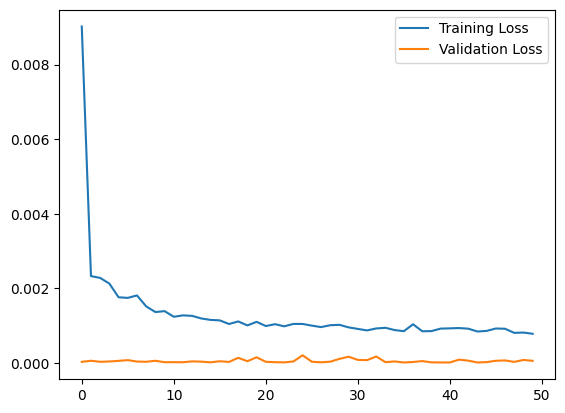
\includegraphics[width=0.9\linewidth]{Wyniki_testowe_i_walidacyjne.png}
    \caption{Wyniki testowe i walidacyjne}
    \label{fig:Wyniki_testowe_i_walidacyjne}
\end{figure}

\paragraph{Wnioski}
Po wykresie widać, że strata na zbiorze treningowym szybko maleje, co może wskazywać na efektywne uczenie się modelu na danych treningowych. Jednak strata na zbiorze walidacyjnym po początkowym spadku, zaczyna się stabilizować. Może to być znakiem, że dochodzi do efektu przeuczenia. Rozwiązaniem tego może być zastosowanie technik regularyzacji takich jak Dropout.

\section{Bezpieczeństwo aplikacji}

Aplikacja wykorzystuje framework \texttt{Spring Security} w celu zapewnienia bezpieczeństwa i kontrolowania dostępu do zasobów. Dzięki zastosowaniu różnych mechanizmów uwierzytelniania i autoryzacji, takich jak \texttt{JWT} (JSON Web Tokens), oraz \texttt{Basic Authentication}, aplikacja jest chroniona przed nieautoryzowanym dostępem. Poniżej przedstawiono kluczowe komponenty zapewniające bezpieczeństwo aplikacji.

\subsection{Konfiguracja bezpieczeństwa} (\texttt{SecurityConfig.java})

Klasa \texttt{SecurityConfig} zawiera pełną konfigurację bezpieczeństwa aplikacji, w tym ustawienia filtrów bezpieczeństwa, które kontrolują dostęp do zasobów. Endpotiny \texttt{/client/register} i \texttt{/client/login}, służą użytkownikowi do rejestracji lub logowania, tak aby mógł mieć dostęp do platformy. 

Klasa ta zawiera również konfigurację \texttt{CORS}, która zezwala na dostęp do zasobów aplikacji z określonych domen (np. \texttt{http://localhost:3000}). Dzięki temu aplikacja ma możliwość komunikacji z frontendem.

\subsection{Generowanie i weryfikacja JWT} (\texttt{JwtTokenUtils.java})

Klasa \texttt{JwtTokenUtils} odpowiedzialna jest za generowanie oraz weryfikację tokenów \texttt{JWT}. Tokeny te są wykorzystywane do uwierzytelniania użytkowników i zapewnienia im dostępu zasobów aplikacji. Klasa ta wykonuje następujące operacje:
\begin{itemize}
    \item Generowanie tokenów \texttt{JWT} z unikalnymi danymi użytkownika.
    \item Weryfikacja ważności tokenu, w tym sprawdzanie daty wygaśnięcia.
    \item Ustalenie, czy użytkownik w tokenie jest tym samym, który jest zapisany w bazie danych.
\end{itemize}
Po weryfikacji tokenu, użytkownik zostaje uwierzytelniony i przypisany do kontekstu bezpieczeństwa aplikacji.

\subsection{Filtrowanie tokenów JWT} (\texttt{JwtAccessTokenFilter.java})

Klasa \texttt{JwtAccessTokenFilter} jest odpowiedzialna za filtrację przychodzących żądań HTTP. Filtr ten sprawdza nagłówek \texttt{Authorization} w żądaniach, aby wyodrębnić i zweryfikować token \texttt{JWT}. Jeśli token jest ważny, uzyskuje dostęp do platformy. W przypadku, gdy token jest nieważny lub nie istnieje, aplikacja zwraca odpowiedź o statusie \texttt{UNAUTHORIZED}.

\subsection{Zarządzanie danymi użytkowników} (\texttt{UserInfoManager.java})

Klasa \texttt{UserInfoManager} implementuje interfejs \texttt{UserDetailsService} i jest odpowiedzialna za załadowanie użytkownika z bazy danych na podstawie nazwy użytkownika. Metoda \texttt{loadUserByUsername} korzysta z repozytorium \texttt{ClientRepository}, aby odnaleźć użytkownika, a następnie dostarcza jego dane do kontekstu bezpieczeństwa aplikacji, co pozwala na uwierzytelnianie.

\subsection{Rekordy RSA} (\texttt{RSAKeyRecord.java})

Klasa \texttt{RSAKeyRecord} przechowuje klucze RSA (publiczny i prywatny), które są wykorzystywane do weryfikacji i generowania tokenów \texttt{JWT}. Klucz publiczny jest używany do weryfikacji podpisu tokenu, natomiast klucz prywatny służy do jego generowania. Jest to istotny element systemu autoryzacji, zapewniający integralność i bezpieczeństwo transmisji danych.

\subsection{Podstawowa autentykacja} (\texttt{BasicAuthenticationSecurityConfiguration.java})

Klasa \texttt{BasicAuthenticationSecurityConfiguration} wprowadza mechanizm podstawowej autentykacji. Choć nie zawiera jeszcze pełnej logiki konfiguracyjnej, jest przygotowana do użycia w przyszłości w celu rozszerzenia mechanizmów uwierzytelniania w aplikacji.	
	
\section{Struktura katalogów w aplikacji frontendowej}

Struktura katalogów w aplikacji frontendowej jest zorganizowana w sposób, który umożliwia łatwą skalowalność i utrzymanie kodu. Poniżej przedstawiono główną strukturę folderów aplikacji, która jest typowa dla aplikacji React.
{\footnotesize
\begin{verbatim}
frontend
|-- node_modules
|-- public
|-- src
    |-- blockchain
        |-- accounts
        |-- blocks
        |-- transactions
    |-- clientOptions
        |-- predictPrices
        |-- simulateTransaction
    |-- cryptocurrency
        |-- categories
        |-- gainersAndLosers
        |-- globalMarket
        |-- historicalData
        |-- ranking
    |-- login
    |-- mainpage
    |-- resources
        |-- converter
        |-- directory
        |-- news
    |-- signup
    |-- tokens
        |-- collections
        |-- nftStatistics
    |-- App.css
    |-- App.js
    |-- App.test.js
    |-- header.css
    |-- header.js
    |-- index.css
    |-- index.js
    |-- logo.svg
\end{verbatim}
}

\subsection{Opis folderów}

\begin{itemize}
    \item \textbf{\texttt{node\_modules/}}: Zawiera zainstalowane zależności.
    \item \textbf{\texttt{public/}}: Zawiera pliki statyczne.
    \item \textbf{\texttt{src/}}: Główny katalog z kodem źródłowym aplikacji.
    \begin{itemize}
        \item \textbf{\texttt{blockchain/}}: Zawiera pliki do obsługi blockchainów (block, account, transaction).
        \item \textbf{\texttt{clientOptions/}}: Zawiera pliki do obsługi przewidywania cen oraz symulowania transakcji.
        \item \textbf{\texttt{cryptocurrency/}}: Zawiera pliki do obsługi kryptowalut.
        \item \textbf{\texttt{login/}}: Zawiera pliki do obsługi logowania.
        \item \textbf{\texttt{mainpage/}}: Zawiera pliki do obsługi głównej strony.
        \item \textbf{\texttt{resources/}}: Zawiera pliki do obsługi konwersji walut, wiadomości oraz dodatkowych zasobów.
        \item \textbf{\texttt{signup/}}: Zawiera pliki do obsługi rejestracji.
        \item \textbf{\texttt{tokens/}}: Zawiera pliki do obsługi tokenów.
        \item \textbf{\texttt{header.js}}: Jest to plik z nagłówkiem, który jest na każdej stronie.
        \item \textbf{\texttt{App.js}}: Główny komponent aplikacji, który pełni rolę kontenera dla pozostałych komponentów.
        \item \textbf{\texttt{index.js}}: Punkt wejścia aplikacji. Jest to miejsce, gdzie aplikacja React jest renderowana na stronie, a także, gdzie inicjalizowane są wszystkie globalne ustawienia, takie jak konfiguracja routera.
    \end{itemize}
\end{itemize}
